%% Results section. Every table body is generated by paper/scripts/make_tables.py.

\subsection{Coverage: every size, both puzzles}
\label{sec:coverage}

\begin{table*}[t]
\caption{Rubik's Square, random states. Columns: number of instances; mean optimal length (exact
BFS, $N\le4$); mean HTM of \Mfour (per-size network, $W{=}4096$), \FiveA and \FiveB on the same
instances; \FiveB's solved fraction, its length divided by $N^2/\ln N$, and its mean time per
state. A superscript gives the solved fraction when below 100\%; ``--'' = not run (no model for that
size), and ``--$^{0/k}$'' = tried, none solved.}
\label{tab:square}
\small
\begin{tabular}{@{}rrrrrrrrr@{}}
\toprule
$N$ & $n$ & optimal & \Mfour & \FiveA & \FiveB HTM\,$\pm$\,95\% CI & \FiveB solved & \FiveB / $(N^2/\ln N)$ & \FiveB time (s) \\
\midrule
3 & 10 & 3.6 & 3.6 & -- & 4.8\,$\pm$\,1.0 & 10/10 & 0.59 & 0.0 \\
4 & 10 & 6.4 & 6.4 & 6.4 & 13.4\,$\pm$\,1.8 & 10/10 & 1.16 & 0.0 \\
5 & 10 & -- & 8.8 & 10.0 & 22.2\,$\pm$\,2.3 & 10/10 & 1.43 & 0.2 \\
6 & 10 & -- & 13.0 & 15.0 & 28.0\,$\pm$\,2.5 & 10/10 & 1.39 & 0.1 \\
7 & 10 & -- & 15.0 & 23.5$^{4/10}$ & 41.8\,$\pm$\,4.4 & 10/10 & 1.66 & 0.2 \\
8 & 10 & -- & 20.4 & 56.4 & 61.6\,$\pm$\,5.4 & 10/10 & 2.00 & 0.6 \\
9 & 10 & -- & -- & 70.0 & 83.2\,$\pm$\,6.1 & 10/10 & 2.26 & 1.0 \\
10 & 10 & -- & -- & 85.5$^{8/10}$ & 103.4\,$\pm$\,6.1 & 10/10 & 2.38 & 1.6 \\
11 & 10 & -- & -- & -- & 121.4\,$\pm$\,7.5 & 10/10 & 2.41 & 3.3 \\
12 & 10 & -- & -- & --$^{0/1}$ & 143.0\,$\pm$\,6.4 & 10/10 & 2.47 & 5.9 \\
13 & 5 & -- & -- & -- & 170.4\,$\pm$\,7.3 & 5/5 & 2.59 & 7.0 \\
14 & 5 & -- & -- & -- & 221.2\,$\pm$\,17.6 & 5/5 & 2.98 & 11.9 \\
15 & 5 & -- & -- & -- & 242.8\,$\pm$\,20.9 & 5/5 & 2.92 & 13.0 \\
16 & 5 & -- & -- & -- & 280.0\,$\pm$\,15.8 & 5/5 & 3.03 & 15.8 \\
17 & 5 & -- & -- & -- & 298.4\,$\pm$\,30.8 & 5/5 & 2.93 & 21.1 \\
18 & 5 & -- & -- & -- & 354.8\,$\pm$\,11.5 & 5/5 & 3.17 & 34.0 \\
19 & 5 & -- & -- & -- & 394.4\,$\pm$\,23.5 & 5/5 & 3.22 & 43.0 \\
20 & 5 & -- & -- & -- & 486.4\,$\pm$\,43.3 & 5/5 & 3.64 & 60.3 \\
\bottomrule

\end{tabular}
\end{table*}

\begin{table}[t]
\caption{Rubik's Cube, random states, \FiveB. Time is wall-clock seconds per state.}
\label{tab:cube}
\small\setlength{\tabcolsep}{4pt}
\begin{tabular}{@{}rrrrrrr@{}}
\toprule
$N$ & $n$ & solved & HTM & QTM & HTM/$(N^2/\ln N)$ & time (s) \\
\midrule
3 & 2 & 52.0 & \textbf{21.0} & \textbf{21.0} & \textbf{21.0} & 31.0 & 2.6 & 0 \\
4 & 2 & 246.0 & 219.0 & \textbf{192.5} & 196.0 & 224.5 & 17.0 & 1 \\
5 & 2 & 452.5 & 319.5 & 258.0 & \textbf{253.0} & 281.0 & 16.3 & 1 \\
6 & 2 & 724.5 & 574.5 & 464.5 & \textbf{437.0} & 481.5 & 21.7 & 4 \\
7 & 2 & 1,045.0 & 811.0 & 633.0 & \textbf{564.0} & 614.5 & 22.4 & 7 \\
8 & 2 & 1,510.5 & 1,131.0 & 897.5 & \textbf{806.5} & 863.0 & 26.2 & 17 \\
10 & 2 & 2,260.5 & 1,900.5 & 1,509.0 & \textbf{1,196.5} & 1,256.5 & 27.6 & 37 \\
15 & 1 & 5,280.0 & 4,565.0 & 3,578.0 & \textbf{2,765.0} & 2,927.0 & 33.3 & 223 \\
20 & 1 & 9,904.0 & 8,259.0 & 6,612.0 & \textbf{4,925.0} & 5,188.0 & 36.9 & 158 \\
\bottomrule

\end{tabular}
\end{table}

\FiveB solved all \SqSolved{} of \SqTotal{} Square instances (Table~\ref{tab:square}) and all
\CuSolved{} of \CuTotal{} cube instances (Table~\ref{tab:cube}). The \Sq{20} took
\SqTwentyTime{}\,s per state on average; the \Cu{15} took \CuFifteenMin{} minutes
(\CuFifteenHTM{} moves) and the \Cu{20} \CuTwentyMin{} minutes (\CuTwentyHTM{} moves). To our
knowledge no earlier learned-search solver has been reported beyond the
\Cu{5}~\cite{chervov2025cayleypy}. The price is length: \FiveB's \Cu{3} solutions average
\CuThreeHTM{} HTM, against an optimum of about 18 on random states~\cite{rokicki2014diameter}.

\subsection{Distance from optimal on small Squares}
\label{sec:optimal}

The \Sq{3} and \Sq{4} are small enough to enumerate. Breadth-first search from all four solved
orientations visits \StatesSquareThree{} and \StatesSquareFour{} states; their diameters are
\GodSquareThree{} and \GodSquareFour{} moves. Table~\ref{tab:optimal} scores each method against
the exact optimum on the same instances. The per-size network of \Mfour found the optimum on every
instance (\OptMfourThree{} and \OptMfourFour{}). \FiveB was \GapFiveBThree{} and \GapFiveBFour{}
moves above it on average: its stages fix pieces in a prescribed order and pay for commutators
that a global search does not need.

\begin{table}[t]
\caption{Optimality on the smallest Squares. ``Gap'' = mean HTM above the exact optimum over
solved instances; ``optimal'' = instances solved in exactly the optimal length. \FiveA was
evaluated for $N\ge4$ only.}
\label{tab:optimal}
\small\setlength{\tabcolsep}{4pt}
\begin{tabular}{@{}lrrlrrr@{}}
\toprule
Puzzle & God's & mean opt. & Method & solved & gap & optimal \\
\midrule
\multirow{3}{*}{3$\times$3} & \multirow{3}{*}{6} & \multirow{3}{*}{3.6} & Method 4 ($W{=}4096$) & 10/10 & 0.0 & 10/10 \\
 & &  & Method 5A & -- & -- & -- \\
 & &  & Method 5B & 10/10 & 1.2 & 1/10 \\
\midrule
\multirow{3}{*}{4$\times$4} & \multirow{3}{*}{10} & \multirow{3}{*}{6.4} & Method 4 ($W{=}4096$) & 10/10 & 0.0 & 10/10 \\
 & &  & Method 5A & 10/10 & 0.0 & 10/10 \\
 & &  & Method 5B & 10/10 & 7.0 & 0/10 \\
\bottomrule

\end{tabular}
\end{table}

\subsection{Comparison with per-size networks}
\label{sec:pernetwork}

\Mfour's per-size networks are the strongest method we have on the sizes where they exist.
On the \PairedMfourN{} Square instances with $3\le N\le8$ that both methods solved, \FiveB's
solutions were on average \RatioFiveBMfour$\times$ as long as \Mfour's at $W{=}4096$
(Table~\ref{tab:square}). As CayleyPy reports for cubes~\cite{chervov2025cayleypy}, wider beams
help (Figure~\ref{fig:m4width}). They also decide coverage at the largest trained size: on the
\Sq{8}, \Mfour solved \MfourEightSolvedWSixteen{} states at $W{=}16$,
\MfourEightSolvedWTwoFiftySix{} at $W{=}256$ and all from $W{=}1024$ on, at
\MfourEightTimeWFourK\,s per state for $W{=}4096$. The cost is a separate model and training run
for every size; we have them only for $N\le8$.

\begin{figure}[t]
\centering
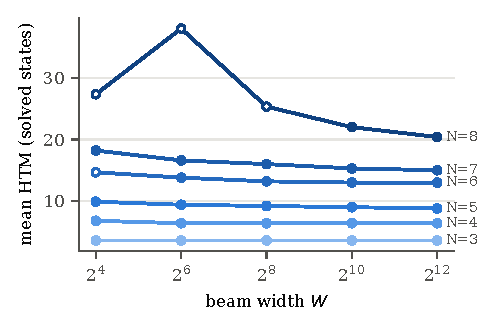
\includegraphics[width=\columnwidth]{figures/m4_width.pdf}
\caption{\Mfour: mean solution length against beam width $W$, one per-size network for each
Square size $N=3,\dots,8$ (10 states each; means over solved states). Hollow markers: not all 10
states solved, so the mean covers only the easier ones.}
\label{fig:m4width}
\end{figure}

\subsection{Does one network generalise across sizes?}
\label{sec:generalisation}

\begin{table}[t]
\caption{\FiveA, trained on Squares with $N\in\{4,\dots,8\}$ only: agreement of its distance
estimate with the true random-walk depth at the end of training, on fresh walks ($^\ast$ = size
never seen in training). RMSE is in units of $N^2/\ln N$.}
\label{tab:gen}
\small\setlength{\tabcolsep}{4pt}
\begin{tabular}{lrrrrrrrr}
\toprule
$N$ & 4 & 5 & 6 & 7 & 8 & 10$^\ast$ & 14$^\ast$ & 20$^\ast$ \\
\midrule
Pearson $r$ & 0.48 & 0.62 & 0.67 & 0.61 & 0.64 & 0.66 & 0.65 & 0.53 \\
normalised RMSE & 0.71 & 0.63 & 0.58 & 0.61 & 0.57 & 0.57 & 0.60 & 0.70 \\
\bottomrule
\end{tabular}

\end{table}

Table~\ref{tab:gen} shows that the distance estimate of \FiveA does not collapse on sizes it never
saw: its correlation with the true walk depth is \FiveACorrEight{} at $N=8$, the largest training
size, \FiveACorrTen{} at $N=10$ and \FiveACorrTwenty{} at $N=20$. These correlations are moderate;
a model of \FiveAParams{} parameters trained for \FiveASteps{} CPU steps is far from converged.

As a solver, \FiveA solved these fractions of instances: \FiveACoverage{}. With full-puzzle beam search it matched or came close
to \Mfour's per-size networks for $N\le6$, including the optimum on all ten \Sq{4} instances
(Table~\ref{tab:optimal}), but at $N=7$ six of ten full-puzzle searches used up their step limit
without reaching the goal: the search horizon, not time, was the problem. Inside
\FiveB's stages ($N\ge8$) it solved most states (the two \Sq{10} failures hit the 300\,s budget), with solutions shorter than \FiveB's own: on the
\PairedFiveAN{} instances both solved, \FiveB's solutions were \RatioFiveBFiveA$\times$ as long as
\FiveA's overall and \RatioFiveBFiveAUnseen$\times$ as long on the \PairedFiveAUnseenN{} instances
with $N>8$, sizes outside \FiveA's training range. The cost is time: transformer scoring on CPU
made \FiveA's staged solves several times slower than \FiveB's (Table~\ref{tab:square}). The one
\Sq{12} we tried did not finish within 900\,s, and we stopped the planned $N=12$ and $N=14$ runs
there; larger sizes need a GPU or a cheaper scoring path such as the move head.

\subsection{Ablations}
\label{sec:ablations}

\begin{table*}[t]
\caption{Ablations of \FiveB, removing one component at a time: macro actions, exact small stages,
the restriction of late center stages to pure-center commutators, the tables-only corner heuristic,
and the coarse abstraction tables (corners then use the MLP alone). Each cell: solved / tried, mean
HTM over solved states, mean seconds per state (failures included in time). Square: 5 states per size, 600\,s budget; cube: 2 states per
size, 300\,s budget. The same instances as Tables~\ref{tab:square} and \ref{tab:cube}.}
\label{tab:ablation}
\small
\begin{minipage}[t]{0.40\textwidth}\centering
\begin{tabular}[t]{@{}lrrrrrr@{}}
\toprule
Square & \multicolumn{3}{c}{$N=8$} & \multicolumn{3}{c}{$N=12$} \\
 & solved & HTM & s & solved & HTM & s \\
\midrule
full \FiveB & 5/5 & 59 & 0.9 & 5/5 & 144 & 4.5 \\
$-$ macros & 5/5 & 59 & 15 & 4/5 & 136 & 111 \\
$-$ exact stages & 5/5 & 67 & 0.5 & 5/5 & 175 & 4.0 \\
\bottomrule
\end{tabular}
\end{minipage}%
\hfill
\begin{minipage}[t]{0.56\textwidth}\centering
\begin{tabular}[t]{@{}lrrrrrr@{}}
\toprule
Cube & \multicolumn{3}{c}{$N=4$} & \multicolumn{3}{c}{$N=5$} \\
 & solved & HTM & s & solved & HTM & s \\
\midrule
full \FiveB & 2/2 & 246 & 31 & 2/2 & 452 & 74 \\
$-$ center restriction & 2/2 & 246 & 41 & 2/2 & 452 & 133 \\
corners: max(MLP, tab.) & 2/2 & 296 & 89 & 2/2 & 421 & 125 \\
$-$ coarse tables & 2/2 & 296 & 87 & 2/2 & 436 & 120 \\
\bottomrule
\end{tabular}
\end{minipage}%

\end{table*}

Table~\ref{tab:ablation} removes one component at a time.

\emph{Macro actions} are what make large Squares fast. Without them the \Sq{8} still solves at the
same length but takes \AblSquareNoMacrosNiTime\,s instead of \AblSquareFullNiTime\,s per state,
and at $N=12$ only \AblSquareNoMacrosNmSolved{} states solve within 600\,s
(\AblSquareNoMacrosNmTime\,s per state against \AblSquareFullNmTime\,s). A commutator turns a
``break, then restore'' detour, which the summed heuristic scores as uphill, into one downhill step.

\emph{Exact small stages} shorten solutions rather than speed them up: solving the frame optimally
instead of by beam search gives \AblSquareFullNiHTM{} instead of \AblSquareNoExactStagesNiHTM{} moves
at $N=8$ and \AblSquareFullNmHTM{} instead of \AblSquareNoExactStagesNmHTM{} at $N=12$.

On the cube, \emph{restricting late center stages to pure-center commutators} left lengths unchanged
here and saved time (\AblCubeFullNfTime\,s against \AblCubeNoCenterMacroRestrictionNfTime\,s per
\Cu{5} state). The \emph{corner heuristic} result is mixed: taking $\max(\text{MLP},\text{tables})$
instead of the tables alone made \Cu{4} solutions longer (\AblCubeCornerMlpPlusTablesNeHTM{}
against \AblCubeFullNeHTM{} moves) and \Cu{5} solutions shorter (\AblCubeCornerMlpPlusTablesNfHTM{}
against \AblCubeFullNfHTM{}), and was slower on both. Removing the coarse tables, so that corners fall back to the MLP alone,
gave the same pattern (\AblCubeNoCoarseTablesNeHTM{} and \AblCubeNoCoarseTablesNfHTM{} moves). With
two states per size we read these cube differences as indicative only; the clearest cube effect is
speed.

\subsection{Scaling with $N$ and lower bounds}
\label{sec:scaling}

\begin{figure*}[t]
\centering
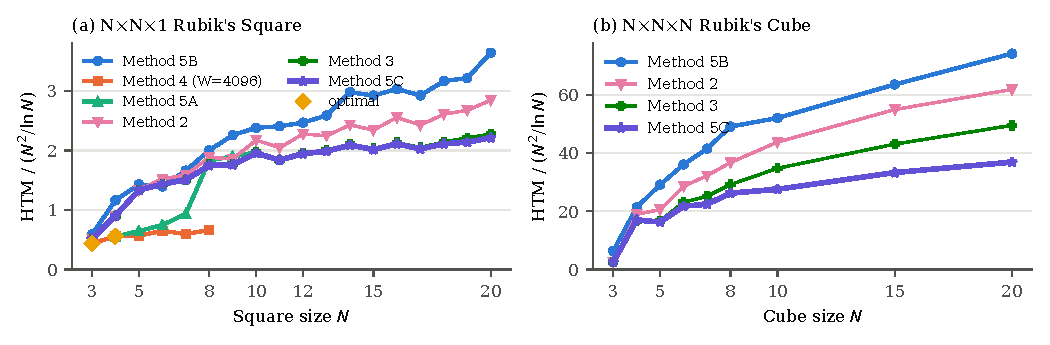
\includegraphics[width=\textwidth]{figures/scaling.pdf}
\caption{Solution length divided by $N^2/\ln N$, the growth rate of the worst case, for the Square
(a) and the cube (b). A flat line would mean growth at the rate of the worst case. Means over solved states;
the same instances as Tables~\ref{tab:square} and \ref{tab:cube}.}
\label{fig:scaling}
\end{figure*}

Figure~\ref{fig:scaling} divides each mean length by $N^2/\ln N$. For \FiveB on the Square this
ratio rises from \SqNormThree{} at $N=3$ to \SqNormTwenty{} at $N=20$, and on the cube it keeps
rising across the whole range. Over the sizes we can test, \FiveB's lengths therefore grow faster
than the $N^2/\log N$ rate that Demaine's construction achieves. The likely cause is that \FiveB
solves clusters a few at a time, while that construction amortises one move sequence over many
identical clusters. The per-size network of \Mfour sits well below
\FiveB where it exists.

\begin{table}[t]
\caption{Counting lower bounds on the worst case (God's number) in our move sets ($2N$ Square flips,
$9N$ cube half-turn moves), from the number of reachable center-cluster configurations as in
Demaine et al.~\cite{demaine2011algorithms}, next to \FiveB's mean length on random states. The
bounds are for the worst state, not for these instances.}
\label{tab:lb}
\small\setlength{\tabcolsep}{4pt}
\begin{tabular}{@{}rrrrr@{}}
\toprule
 & \multicolumn{2}{c}{Square} & \multicolumn{2}{c}{Cube} \\
\cmidrule(lr){2-3}\cmidrule(lr){4-5}
$N$ & lower bound & \FiveB mean & lower bound & \FiveB mean \\
\midrule
6 & 2 & 28 & 35 & 724 \\
8 & 5 & 62 & 75 & 1,510 \\
10 & 9 & 103 & 126 & 2,260 \\
15 & 18 & 243 & 262 & 5,280 \\
20 & 39 & 486 & 557 & 9,904 \\
\bottomrule

\end{tabular}
\end{table}

Table~\ref{tab:lb} puts the counting bounds next to our lengths. The bounds only say that
\emph{some} state needs that many moves, so they cannot certify optimality of any single solution,
but on the cube our lengths are more than an order of magnitude above them, so either the bounds
are very weak or there is much room left; both are likely.
